\documentclass{ximera}
%handout:  for handout version with no solutions or instructor notes
%handout,instructornotes:  for instructor version with just problems and notes, no solutions
%noinstructornotes:  shows only problem and solutions

%% handout
%% space
%% newpage
%% numbers
%% nooutcomes

%I added the commands here so that I would't have to keep looking them up
%\newcommand{\RR}{\mathbb R}
%\renewcommand{\d}{\,d}
%\newcommand{\dd}[2][]{\frac{d #1}{d #2}}
%\renewcommand{\l}{\ell}
%\newcommand{\ddx}{\frac{d}{dx}}
%\everymath{\displaystyle}
%\newcommand{\dfn}{\textbf}
%\newcommand{\eval}[1]{\bigg[ #1 \bigg]}

%\begin{image}
%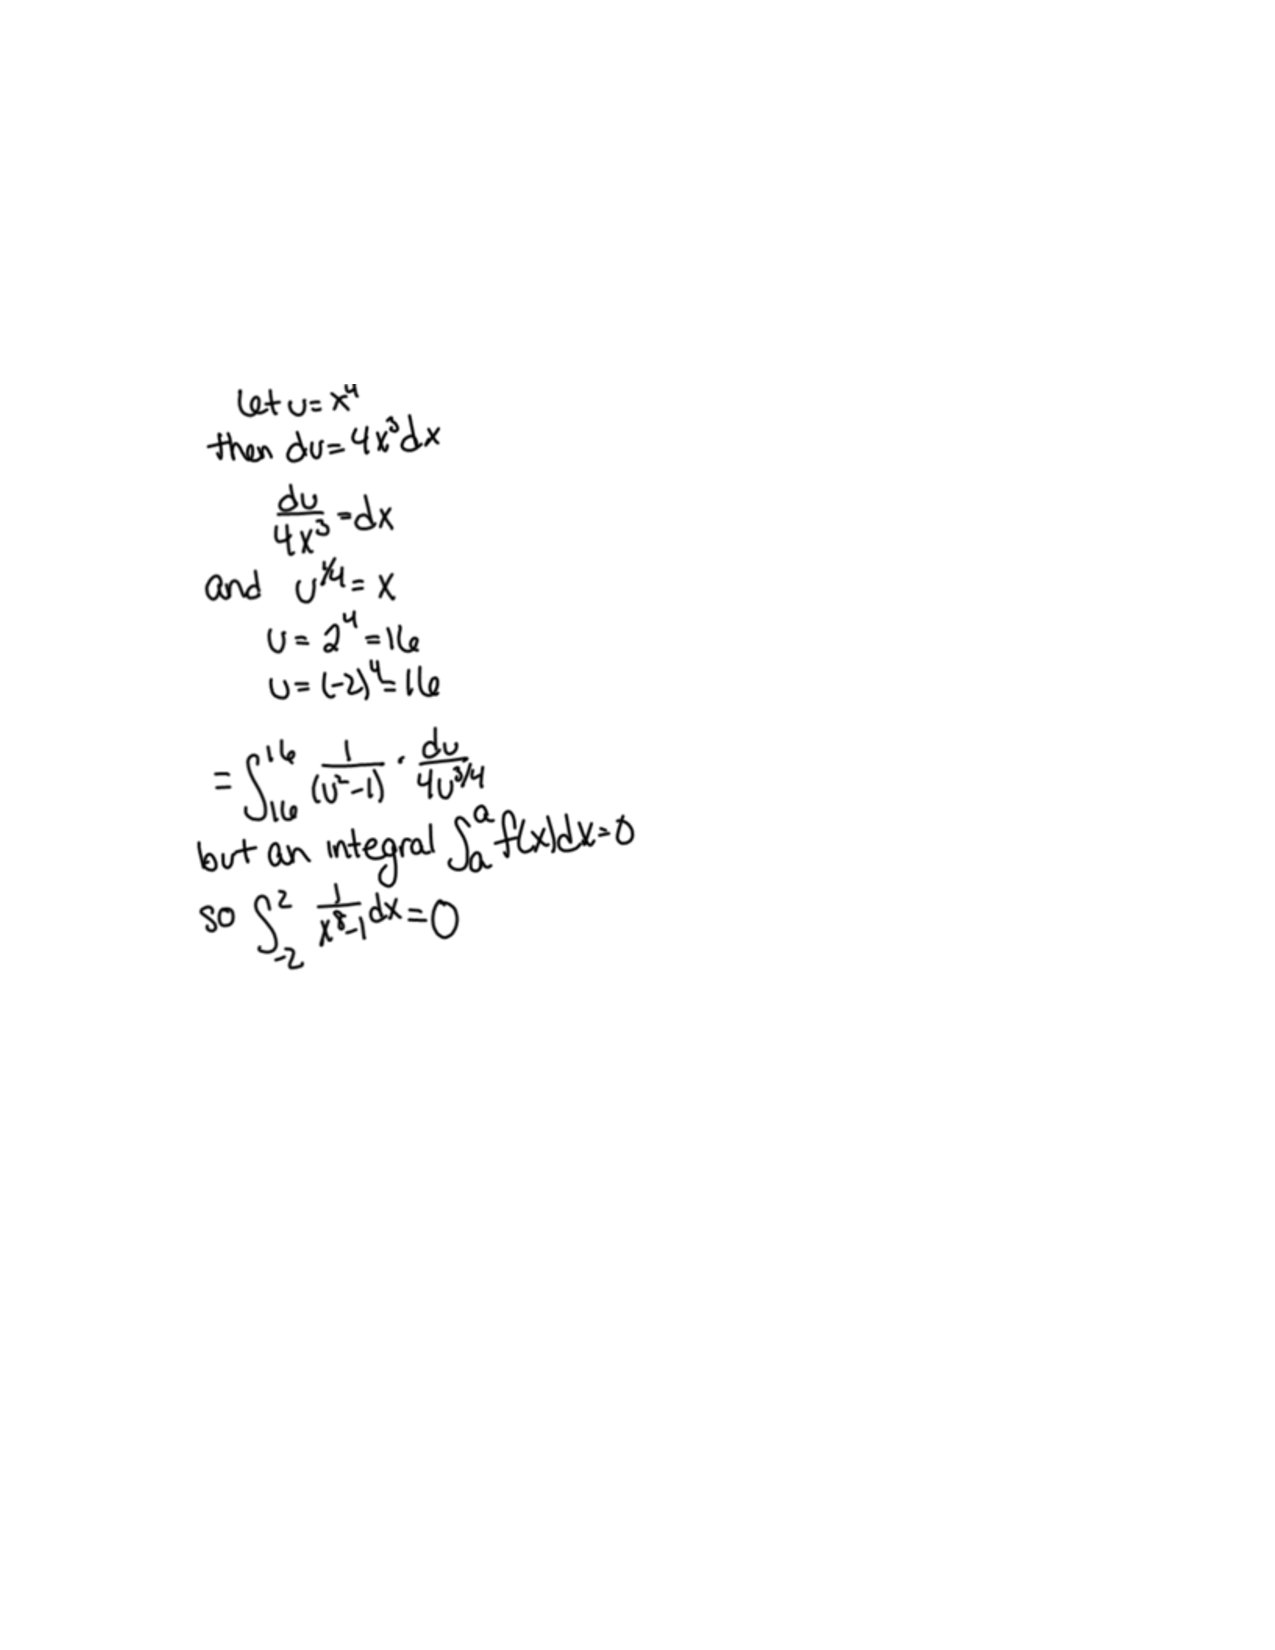
\includegraphics[trim= 170 420 250 180]{Figure1.pdf}
%\end{image}

%add a ``.'' below when used in a specific directory.
\newcommand{\RR}{\mathbb R}
\renewcommand{\d}{\,d}
\newcommand{\dd}[2][]{\frac{d #1}{d #2}}
\renewcommand{\l}{\ell}
\newcommand{\ddx}{\frac{d}{dx}}
\newcommand{\dfn}{\textbf}
\newcommand{\eval}[1]{\bigg[ #1 \bigg]}

\usepackage{multicol}

\renewenvironment{freeResponse}{
\ifhandout\setbox0\vbox\bgroup\else
\begin{trivlist}\item[\hskip \labelsep\bfseries Solution:\hspace{2ex}]
\fi}
{\ifhandout\egroup\else
\end{trivlist}
\fi} %% we can turn off input when making a master document

\title{}  

\begin{document}
\begin{abstract}		\end{abstract}
\maketitle





%\section{Group work:}



%problem 1
\begin{problem}
	\begin{enumerate}
	\item  Show that 
		\begin{equation*}
		\frac{9}{2x^2+3x} = \frac{3}{x} - \frac{6}{2x+3}
		\end{equation*}
	
	\item  Determine if the integral
		\begin{equation*}
		\int_1^\infty \frac{9}{2x^2+3x} \d x
		\end{equation*}
	converges or diverges.  If it converges, give the value that it converges to.
	
	
	
	\begin{freeResponse}
	\begin{enumerate}
	\item
	Since $2x^2+3x = x(2x+3)$, we apply the method of partial fractions:
		\begin{align*}
		&\frac{9}{2x^2+3x} = \frac{A}{x} + \frac{B}{2x+3}  \\
		\Longrightarrow \qquad &9 = A(2x+3) + Bx.
		\end{align*}
	Letting $x=0$ gives that
		\begin{equation*}
		9 = 3A	\quad	\Longrightarrow \quad	A = 3.
		\end{equation*}
	Then letting $x = -\frac{3}{2}$, we see that
		\begin{equation*}
		9 = - \frac{3}{2} B \quad \Longrightarrow \quad B = - 9 \cdot \frac{2}{3} = -6.
		\end{equation*}
	Therefore, plugging in our values for $A$ and $B$ gives us
		\begin{equation*}
		\frac{9}{2x^2+3x} = \frac{3}{x} - \frac{6}{2x+3}.
		\end{equation*}
		
		
		
	\item We have that
		\begin{align*}
		\int_1^\infty \frac{9}{2x^2+3x} \d x &= \lim_{t \to \infty} \int_1^t \left( \frac{3}{x} - \frac{6}{2x+3} \right) \d x  \\
		&= \lim_{t \to \infty} \eval{3\ln|x| - \frac{6}{2} \ln|2x+3|}_1^t  \quad {\color{red}\text{don't forget to divide the 6 by 2}}  \\
		&= \lim_{t \to \infty} \left( 3\ln|t| - 3\ln|2t+3| - 0 + 3\ln(5) \right)  \quad {\color{red}\ln(1) = 0} \\
		&= \lim_{t \to \infty} \left( 3 \ln \left| \frac{5t}{2t+3} \right| \right)  \quad {\color{red}\text{properties of logarithms}}  \\
		&= \boxed{3 \ln \left( \frac{5}{2} \right)}	\quad	{\color{red}\text{since ln(x) is a continuous function}}
		\end{align*}
	
	\end{enumerate}
	\end{freeResponse}
	
	\end{enumerate}
	
		
\end{problem}












%problem 2
\begin{problem}
		\begin{enumerate}
	\item  Show that 
		\begin{equation*}
		\frac{6x-8}{x^3+4x} = \frac{2x+6}{x^2+4} - \frac{2}{x}
		\end{equation*}
	
	\item  Determine if the integral
		\begin{equation*}
		\int_3^\infty \frac{6x-8}{x^3+4x} \d x
		\end{equation*}
	converges or diverges.  If it converges, give the value that it converges to.
	
	
	
	\begin{freeResponse}
	\begin{enumerate}
	\item
	Since $x^3+4x = x(x^2+4)$, we use partial fractions:
		\begin{align*}
		&\frac{6x-8}{x^3+4x} = \frac{Ax+B}{x^2+4} + \frac{C}{x}  \\
		\Longrightarrow 	\qquad	&6x-8 = (Ax+B)(x) + C(x^2+4).
		\end{align*}
	Letting $x=0$, we see that
		\begin{equation*}
		-8 = 4C \quad \Longrightarrow \quad C = -2.
		\end{equation*}
	To find $A$ and $B$, let us plug in $C=-2$ and simplify:
		\begin{align*}
		6x-8 &= Ax^2 + Bx -2x^2 - 8  \\
		&= (A-2)x^2 + Bx - 8.
		\end{align*}
	Aligning the respective coefficients, we see that
		\begin{align*}
		&A-2 = 0	\quad	\text{and}	\quad	B=6  \\
		\Longrightarrow		\quad	&A=2	\quad	\text{and}	\quad	B=6.
		\end{align*}
	Finally, plugging this into the original equation yields
		\begin{equation*}
		\frac{6x-8}{x^3+4x} = \frac{2x+6}{x^2+4} - \frac{2}{x}.
		\end{equation*}
		
		
		
		
	\item We have that
		\begin{align*}
		\int_3^\infty \frac{6x-8}{x^3+4x} \d x &= \lim_{t \to \infty} \int_3^t \left( \frac{2x+6}{x^2+4} - \frac{2}{x} \right) \d x  \\
		&= \lim_{t \to \infty} \left( \int_3^t \frac{2x}{x^2+4} \d x + \int_3^t \frac{6}{x^2+4} \d x - \int_3^t \frac{2}{x} \d x \right).
		\end{align*}
	Let us evaluate each integral separately, combine them, and then take the limit.
	
		\begin{enumerate}
		\item[(i)]  \begin{align*}
		\int_3^t \frac{2x}{x^2+4} \d x &= \int_{13}^{t^2+4} \frac{1}{w} \d w	\quad	{\color{red}w=x^2+4, \d w = 2x \d x}  \\
		&= \ln(t^2 +4) - \ln(13).
		\end{align*}
		
		\item[(ii)]  \begin{align*}
		\int_3^t \frac{6}{x^2+4} \d x &= \eval{\frac{6}{2} \arctan \left( \frac{x}{2} \right) }_3^t  \\
		&= 3 \arctan \left(\frac{t}{2} \right) - 3 \arctan \left( \frac{3}{2} \right).
		\end{align*}
		
		\item[(iii)]  \begin{align*}
		\int_3^t \frac{2}{x} \d x &= \eval{ 2 \ln|x| }_3^t  \\
		&= 2 \ln|t| - 2\ln(3).
		\end{align*}
		
		\end{enumerate}
	We now combined these three expressions, and then compute the limit.
		\begin{align*}
		&\int_3^\infty \frac{6x-8}{x^3+4x} \d x  \\
		&= \lim_{t \to \infty} \left[ \left(\ln(t^2 +4) - \ln(13) \right) + \left( 3 \arctan \left(\frac{t}{2} \right) - 3 \arctan \left( \frac{3}{2} \right) \right) - \left( 2 \ln|t| - 2\ln(3) \right) \right]  \\
		&= \lim_{t \to \infty} \left[ \ln(t^2+4) - \ln t^2 + 3 \arctan \left( \frac{t}{2} \right) - \ln 13 + \ln 9 - 3 \arctan \left( \frac{3}{2} \right) \right]  \\
		&= \lim_{t \to \infty} \left[ \ln \left( \frac{t^2+4}{t^2} \right) + 3 \arctan \left( \frac{t}{2} \right) - \ln 13 + \ln 9 - 3 \arctan \left( \frac{3}{2} \right) \right]  \\
		&= \ln(1) + 3 \cdot \frac{\pi}{2} - \ln 13 + \ln 9 - 3 \arctan \left( \frac{3}{2} \right) 	\quad	{\color{red}\lim_{t \to \infty} \arctan(t) = \frac{\pi}{2}}\\
		&= \boxed{\frac{3\pi}{2} - \ln 13 + \ln 9 - 3 \arctan \left( \frac{3}{2} \right)}	\quad	{\color{red}\text{if you like, }- \ln 13 + \ln 9 = \ln \left( \frac{9}{13} \right)}
		\end{align*}
	
	\end{enumerate}
	\end{freeResponse}
	
	\end{enumerate}
\end{problem}











	
	
	
	
	
	
	
	
	

	










								
				
				
	














\end{document} 


















